\documentclass{report}
\usepackage[utf8]{inputenc}
\usepackage{graphicx}
\usepackage{longtable}
\usepackage{array}
\usepackage{caption}
\usepackage{mathtools}
\usepackage{listings}

\pagestyle{headings}

\title{Effects of the EPNs and FLPs on the Information Node for ALICE\\Cern}
\author{M.Q Puls}
\date{2018}

\begin{document}
\lstset{language=Python}

\maketitle

\newpage

\resizebox{\textwidth}{!}{\begin{tabular}{| l | l |}
\hline
Title & Effects of the EPNs and FLPs on the Information Node for ALICE \\ \hline
Name & Mitchell Quinn Puls \\ \hline
Student Number & 500659986 \\ \hline
Phone & +31615050310 \\ \hline
Email & mitchpuls@upcmail.nl \\ & mitch.puls@hva.nl \\ \hline
Place & Amsterdam \\ \hline
Date & 2018 \\ \hline
University & University of Applied Sciences Amsterdam \\ \hline
Department & TI \\ \hline
Mentor & C. J. Rijsenbrij \\ \hline
Company & University of Amsterdam \\ & Software for Science \\ & Wibautstraat 2-4 Amsterdam \\ & 0205995555 \\ \hline
Company Supervisor & Dr. Marten Teitsma \\ \hline
Period & Feb. 2018 - Jul 2018 \\ 
\hline
\end{tabular}}

\newpage

\begin{center}
\section*{Preface}
%This report is a representation of the hard times through my study. It is the product of my ups and downs. Without the support of my teachers at the Amsterdam University of Applied Science, I would not be here where I am now, but by foremost I would like to dedicate this report to my girlfriend Julia Klu{\ss}meier. Who for the last two years was at the forefront of all my stress and frustrations.\\~\\
Mitchell Quinn Puls
\end{center}

\newpage

\tableofcontents

\newpage

\chapter*{Summary}

\newpage

\chapter{Introduction}

This research is conducted as part of the final thesis of Mitchell Quinn Puls, Technical Computing student at the Amsterdam University of Applied Sciences. This research is about the effects of a high amount of computers, processing a vast amount of data. This research is, in assignment from CERN in Switzerland. 
\section{CERN}
CERN is a European organization for  nuclear research, situated in Geneve Switzerland. CERN was founded in 1954 and is one of Europe's first joint ventures. The main goal is to study the fundamental structure of the universe, by researching matter and particles using purpose built particle accelerators and detectors. Particle accelerators beam particles to high energies, before colliding them against each other against or a stationary object. Detectors record and observe this collision (About Cern, 2012). One of these detectors is ALICE
\section{ALICE}
ALICE stands for A Large Ion Collider Experiment, and is a detector mounted on the Large Hadron Collider at CERN.  ALICE's main function is to study matter at extreme energy densities, where matter turns into a form called quark-gluon plasma. Everything in the universe is made from protons, neutrons (except hydrogen which does not have any neutrons) and electrons. Protons and neutrons are then build up with quarks and bound together with something called a gluon. Quark-gluon plasma is matter that appeared at the very start of the big bang, and is the matter that appears when the quarks and gluons are seperated from each other. CERN wants to observe this matter. The way they achieve this, is by shooting two lead ions against each other. This produces heat that is over 100,000 times hotter than the center of the Sun. This breaks the bounds between the quarks and the gluons and makes the quark-gluon plasma visible. (ALICE, 2012)
\subsection{Upgrade}
In July 2018 the accelerator will be stopped for around 18 months for a planned upgrade of the ALICE detector. (van der Lee, 2017, p. 1) During this period, CERN is upgrading it's hardware and software. This upgrade is in collaboration with various schools and universities throughout Europe, including the Amsterdam University of Applied Science. One of these upgrades is an algorithm for Load Balancing. In 2020, ALICE will restart with it's new upgraded detector. ("Technical Design Report for the Upgrade of the Online Offline Computing System", 2015, p. i)

\section{Load Balancing}
The data stream that comes from ALICE is equal to about 1.1 Terabyte per second. All of this data comes in what is known as a heartbeat. This heartbeat gets distributed over 250 First Level Processors and funneled through	1500 Event Processing Nodes. The efficient distribution of this process, and also the handling of data in case of a failure in the system, is what is known as Load Balancing. All of these computers are monitored by an Information Node.

\chapter{Framework}

This chapter will go more in depth about the several different kinds of hardware and software used. It will also elaborate on the different terms and names used for aspects of the research.
\section{$O^2$ Balancer}
$O^2$ Balancer is a framework used by CERN for simulation experiments for ALICE. The code is open source and licensed under the GNU General Public License V3.0. (GNU General Public License v3.0, 2007)

\subsection{Devices}
The $O^2$ Balancer consist of a cluster of 1750 computers, divided in 250 First Level Processors (FLPs) and 1500 Event  Nodes (EPNs) These computers are meant to process the data stream coming from ALICE. All of these computers are monitored using an Information Node.

\subsubsection*{First Level Processors}
The FLPs are the first computers in the line. They receive the data stream (approximately 1.1TB/s) from ALICE and need to distribute that to the next line of computer. In order to do that it takes the data received between two heartbeats, and compresses that into something that's called a Sub Timeframe (STF). A heartbeat lasts for about 20ms. It will then send this STF to the next line of computers which are the EPNs. Every EPN needs to get the same amount of STFs at the same time for recreation purposes. These STFs can then be further examined from there.("Technical Design Report for the Upgrade of the Online Offline Computing System", 2015, p. 33)

\subsubsection*{Event Processing Nodes}
The next line of computers are the EPNs. These receive the STFs from the FLPs and then compress them back into a time frame (TF). This compression reduces it's size by a factor of eight. These TFs are then stored for further use and examination.("Technical Design Report for the Upgrade of the Online Offline Computing System", 2015, p. 33)

\subsubsection*{Information Node}
There is one final computer which is the Information Node (IN). This computer keeps track of all the FLPs and EPNs that are online and makes sure that FLPs don't send data to offline EPNs. ("Technical Design Report for the Upgrade of the Online Offline Computing System", 2015, p. 34)

\begin{figure}
	\centering
	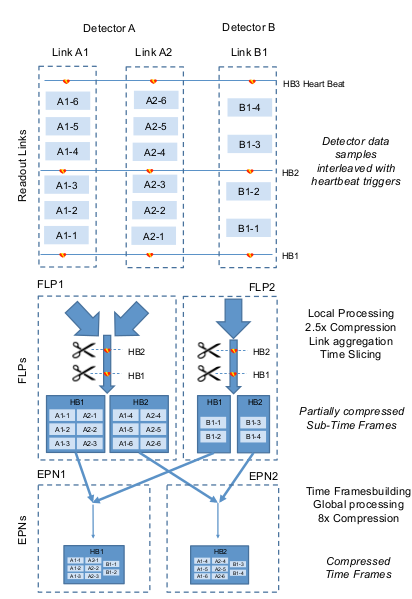
\includegraphics[scale=1]{./graphics/data_aggregation.png}
	\caption{Aggregation of data ("Technical Design Report for the Upgrade of the Online Offline Computing System", 2015, p. 34)}
\end{figure}

\section{FairMQ}
The transport layer used for the $O^2$ Balancer is FairMQ. This is a transport layer from the larger framework FairRoot \footnote{https://github.com/FairRootGroup/FairRoot} created by GSI Darmstadt. In order to accommodate the smaller processing size of the Raspberry Pi, a trimmed down version of FairRoot is used which is just FairMQ. This is a data transport layer used to send data in between the IN, FLPs and EPNs. 
\subsection{Splitting off FairMQ}
During this report, the FairMQ repository had to be split off from FairRoot still. In the first stages of the prototype an emergency version was used made by Heiko van der Heijden. Meanwhile a pull request 
\footnote{https://github.com/FairRootGroup/FairRoot/issues/736} was done on the FairRoot github which resulted in the official FairMQ repository.

\section{Zookeeper}
Zookeeper is a program made by Apache to regulate the whole load balancing process. It is run on the Information Node and from there pings to all EPNs to check whether they are online or not. It then creates a list of online EPNs which it gives to the FLPs so that they know to what EPN to send data to. The frequency of these pings are called the Ticktime. 

\section{Fail-over}
When an EPN goes offline it is called a Fail-over. When this happens, Zookeeper will know that it is offline and will notify the FLPs to not send any data to this EPN anymore. 

\section{Ansible}
Ansible is a deployment software used to create simple automation for large infrastructures. This is used to automate repetitive task for the experiment, and for deploying software stacks to every unit. 

\section{Blacklist Algorithm}
The algorithm used in the previous experiment is a Blacklist Algorithm. This algorithm constantly keeps a list of online channels which is updated by the Information Node using Zookeeper. Once Zookeeper realizes that an EPN is offline, it will update the list so that the algorithm will skip that offline EPN. With this list of online EPNs, the algorithm uses a Round Robin approach to distribute the STF over the EPNs. A way to implement the Blacklist algorithm is shown in figure ~\ref{fig:BlacklistAlgorithm}

\begin{figure}[htb]
	\centering
	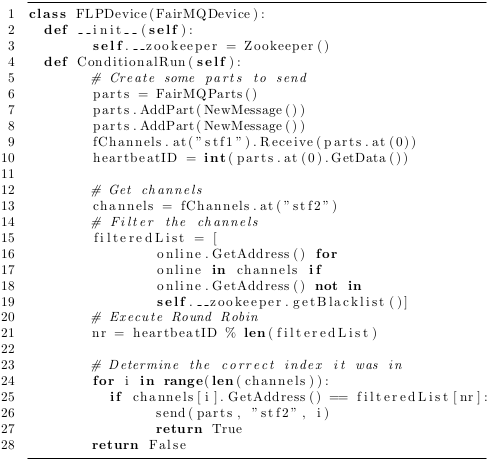
\includegraphics[scale=0.6]{./graphics/BlacklistAlgorithm.png}
	\caption{Blacklist algorithm as it could be implemented in Python (van der Heijden, 2018, p. 20)}
	\label{fig:BlacklistAlgorithm}
\end{figure}


\section{Raspberry Pi}
Raspberry Pi is a  low cost small computer used for prototyping projects \footnote{https://www.raspberrypi.org/about/}. These projects go from small sensor applications, to bigger host-server applications. The Raspberry Pi used for this research is the model 3 B+ variant. As of the time this report is written this is the latest version released. This model is used because of the high Ethernet speeds on the board itself. The reason a Raspberry Pi was used for this experiment is because it's a smaller and cheaper alternative compared to what the cluster on Nikhef used. (van der Heijden, 2018, p. 21) and because of this, it is more easily expanded.

\chapter{Experiments}

This chapter goes more in depth of the specifics on the experiments conducted. It describes the exact hardware specifications and software libraries used. It also defines all the different experiments and includes several figures for added information.
\section{Hardware}
The hardware used for this experiment are specially designed clusters made with Raspberry Pi's 3 model B+. These Pi's are assigned using the same ratio of FLPs and EPNs at CERN (1:6) and 1 Information Node. The Pi's are modified with an extra Ethernet port. The exact specifications are in table 5.1:

\begin{table}[htb]
\begin{tabular}{| l | l |}
\hline
Processor & Cortex-A53 1.4GHZ\\ \hline
RAM & 1GB LPDDR2 SDRAM\\ \hline
Network & 1 300MbE 1 10/100MbE \\ \hline
Operating System & Raspbian Stretch (Debian 9)\\ \hline
\end{tabular} 
\caption{Specifications modified Raspberry Pi 3 model B+}
\end{table}

Everything is setup and built from a single server unit. The IP addresses are also managed from this unit. Specifications are in table 5.2:

\begin{table}[htb]
\begin{tabular}{| l | l |}
\hline
Processor & Intel Xeon\\ \hline
RAM & \\ \hline
Network & \\ \hline
Operating System & Raspbian Stretch (Debian 9)\\ \hline
\end{tabular}
\caption{Specifications management server}
\end{table}

\newpage

The network configuration consists of a bidirectional connection of :
\begin{figure}[htb]
    \centering
    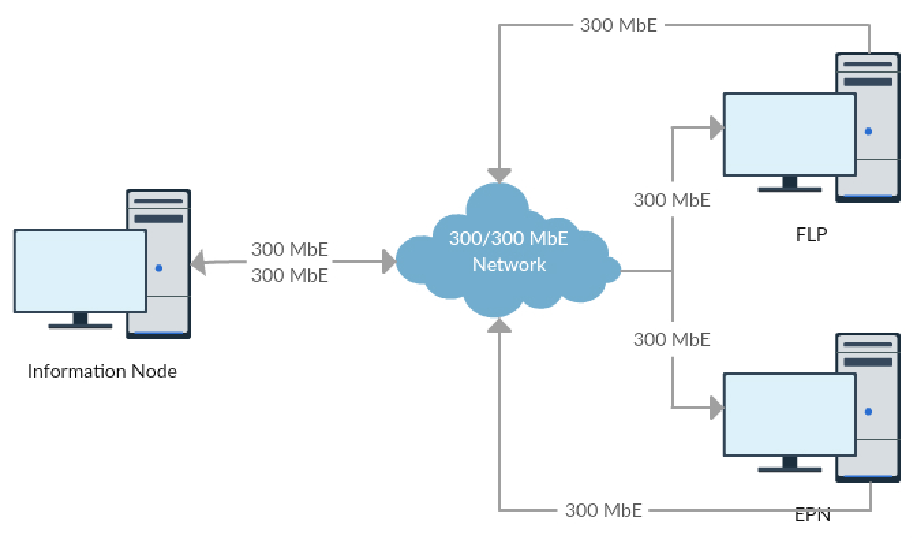
\includegraphics[scale=0.5]{./graphics/chapter5/Network_thesis.pdf}
    \caption{Network setup}
\end{figure}

\newpage

The clusters of pi's are build using a 

\section{Software}
The software used is found at https://github.com/SoftwareForScience/O2-Balancer. It consists of 3 executable programs to represent an FLP, EPN and Information Node. These programs are send to the devices to represent their respective units. Apart from that it uses a slightly modified version of FairRoot
\footnote{https://github.com/FairRootGroup/FairRoot}. 
Since only the FairMQ
\footnote{https://github.com/FairRootGroup/FairMQ}
 part is needed for the programs to run it has been split off from this code.\\
The Infomation Node serves two purposes. At first it generates the TFs that are send to the FLPs using FairMQ. It also receives notifications from the EPNs when they have received the full TF from the FLPs again. The configuration is done using YAML files. A diagram of the connections and dependencies are as followed.

%\begin{figure}[htb]
%    \centering
%    \textbf{Your title}\par\medskip
%    \includegraphics[scale=0.3]{}
%    \caption{Block diagram of the cluster connections (van der Heijden, 2018, p. 22)}
%\end{figure}

\begin{table}[htb]
\begin{tabular}{| l | l |}
\hline
Library/Tool & Version \\ \hline
FairMQ & 1.1.5\\ \hline
ZeroMQ & 4.2.1\\ \hline
Zookeeper & 3.4.9 \\ \hline
Cmake & 3.11.0 \\ \hline
Boost & 1.66.0 \\ \hline
Yaml-cpp & 0.5.2 \\ \hline
Compiler & gcc 6.3.0 20170516 (Raspbian 6.3.0-18+rpi1+deb9u1)\\ \hline
\end{tabular}
\caption{Dependencies software}
\end{table}

\section{Data analysis tools}
In order to stay consistent with the previous experiment, the same tools will be used to create and visualize the data. This can be found at \\ https://github.com/valvy/BalancerScripts. These scripts are written in Python and ROOT to generate graphs and histograms from the log files received from the software. The dependencies are specified in table 5.4.

\begin{table}[ht]
\begin{tabular}{| l | l |}
\hline
Tool & Version \\ \hline
Raspbian & Centos 7 \\ \hline
ROOT & 6.13.02 \\ \hline
Python & 2.7.13 \\ \hline
Ansible & 2.2.1 \\ \hline
\end{tabular}
\caption{Dependencies for the analysis scripts}
\end{table}

\newpage

\section{Experiments}
In order to check whether or not the Information Node has any issues with increased numbers of FLPs and EPNs, the same experiments need to be done as described in the previous report (van der Heijden, 2018, p23-p27) but will be briefly summarized again. The experiments are done in two steps. At first the experiments need to be run using the same amount of FLPs and EPNs to verify whether or not the new setup of Pi clusters are able to give the same result. After that the experiments need to be run again using more FLPs and EPNs to check if it indeed does have an effect on the Information Node.

\subsection{Experiment one}
\textbf{Ticktime influence on the Blacklist algorithm with one fail-over.}
\\\\
The first experiment uses a fixed sample size to be sent from the Information Node, and will have 1 fail-over during its run. This sample size is set to hundred-forty kilobyte and 
the heartbeat rate is set to twenty milliseconds. This heartbeat is set at the same rate used at CERN. This sample size is set to accommodate the slower Ethernet and processing speed of Raspberry Pi as compared to units used in the previous experiment (van der Heijden, 2018, p.23). \\
This experiment will disable one EPN when it recieves the first STF from hearbeat 3.000. Then special scripts will parse the logfiles between heartbeat 2.000 and 10.000 to have enough of a buffer to read from. A flowchart can be found in figure 5.3.

%\begin{figure}[htb]
%    \centering
%    \textbf{Your title}\par\medskip
%    \includegraphics[scale=0.3]{}
%    \caption{Flow char experiment (van der Heijden, 2018, p. 24)}
%\end{figure}

\subsection{Experiment two}
\textbf{Ticktime influence on the Blacklist algorithm with all but one fail-over.}
\\\\
The same heartbeat rate and sample size are used from experiment one. For this experiment the first EPN will disabled at heartbeat 2.000. After that every 1.000 heartbeats an additional EPN will be disabled until there is only 1 left. Scripts will parse all the logs to check how many TFs were lost during this progress. A flowchart can be found in figure 5.4.

%\begin{figure}[htb]
%    \centering
%    \textbf{Your title}\par\medskip
%    \includegraphics[scale=0.3]{}
%    \caption{Flow chart random init experiment (van der Heijden, 2018, p. 25)}
%\end{figure}

\subsection{Experiment three}
\textbf{Ticktime influence on the Blacklist algorithm with all but one fail-over with random sample size.}
\\\\
The same heartbeat rate is used from experiment one. A random sample size will be generated from the FLPs between .. \& .. . Apart from that the same configuration will be used as in experiment two. The first EPN will be disabled at heartbeat 2.000 and after that every 1.000 heartbeats an additional EPN will be disabled. A flowchart can be found in figure 5.5.

%\begin{figure}[htb]
%    \centering
%    \textbf{Your title}\par\medskip
%    \includegraphics[scale=0.3]{}
%    \caption{Flow chart random experiment (van der Heijden, 2018, p. 26)}
%\end{figure}

\subsection{Experiment four}
\textbf{Ticktime influence on the Blacklist algorithm with all but one fail-over at once.}
\\\\
The same heartbeat rate is used from experiment one. For this experiment all but one EPN will be disabled at heartbeat 3.000. After that the system will run for another 7.000 heartbeats to get enough of a buffer to read from. A flowchart can be found in figure 5.6.

\chapter{Results}

\section{Ex.1 2 FLPs 12 EPNs}
\textbf{Ticktime influence on the Blacklist algorithm with one fail-over.}
\\~\\
The results of the experiment are shown in table ~\ref{table:Ex1MitchResults}. It shows that there is a linear line going up with the amount of TFs lost compared to ticktime. It also shows that the mean and standard deviation at ticktime 20 are round. This would be because of the ticktime being in sync with the heartbeat rate.

\begin{table}[h!]
\caption*{\textbf{Experiment one (2/12) using a cluster of Raspberry Pi's}}
\begin{tabular}{| l | l | l |}
\hline
Ticktime & Mean TF loss & Standard Deviation \\ \hline
5 & 2.16 & 0.49 \\ \hline
10 & 2.13 & 0.47 \\ \hline
15 & 3.08 & 0.2 \\ \hline
20 & 3.0 & 0 \\ \hline
25 & 3.52 & 0.51 \\ \hline
30 & 4.32 & 0.57 \\ \hline
35 & 4.13 & 0.79 \\ \hline
40 & 4.56 & 0.16 \\ \hline
\end{tabular}
\caption{Results of the TFs lost with 1 fail over using a cluster of Raspberry Pi's}
\label{table:Ex1MitchResults}
\end{table}

~\\ If we compare this to the previous experiment shown in table ~\ref{table:Ex1HeikoResults}, we can see that there is a small difference in the mean of the TFs lost, and some small variations in the standard deviation.

\begin{table}[h!]
\caption*{\textbf{Experiment one (2/12) using a cluster on Nikhef}}
\begin{tabular}{| l | l | l |}
\hline
Ticktime & Mean TF loss & Standard Deviation \\ \hline
5 & 1.24 & 0.4271 \\ \hline
10 & 1.84 & 0.731 \\ \hline
15 & 2.16 & 0.3666 \\ \hline
20 & 2.12 & 0.325 \\ \hline
25 & 2.708 & 0.4545 \\ \hline
30 & 3 & 0 \\ \hline
35 & 3.52 & 4.996 \\ \hline
40 & 3.76 & 0.4271 \\ \hline
\end{tabular}
\caption{Results of the TFs lost with 1 fail over using a cluster of Intel Xeons (van der Heijden, 2018, p. 36)}
\label{table:Ex1HeikoResults}
\end{table}

\section{Ex.2 2 FLPs 12 EPNs}
\textbf{Ticktime influence on the Blacklist algorithm with all but one fail-over.}
\\~\\
Table ~\ref{table:Ex2MitchResults} shows the lost TFs per ticktime/EPN ratio. For every extra EPN that is lost, the lost TFs increase in a linear motion. This is compliant with the previous experiment. These results are shown in table ~\ref{table:Ex2HeikoResults}. A histogram of ticktime 5 shown at ~\ref{Ex2Histogram} shows that the standard deviation is 0.9568.

\begin{table}[h!]
\caption*{\textbf{Experiment two (2/12) using a cluster of Raspberry Pi's}}
\resizebox{\textwidth}{!}{\begin{tabular}{| p{0.1\linewidth} | >{\centering}m{0.7cm} | >{\centering}m{0.7cm} | >{\centering}m{0.7cm} | >{\centering}m{0.7cm} | >{\centering}m{0.7cm} | >{\centering}m{0.7cm} | >{\centering}m{0.7cm} | >{\centering}m{0.7cm} | >{\centering}m{0.7cm} | >{\centering}m{0.7cm} | >{\centering}m{0.7cm} | >{\centering}m{0.7cm} |}
\hline
Lost EPNs & 1 EPN & 2 EPNs & 3 EPNs & 4 EPNs & 5 EPNs & 6 EPNs & 7 EPNs & 8 EPNs & 9 EPNs & 10 EPNs & 11 EPNs & Total \tabularnewline \hline
Ticktime &&&&&&&&&&&& \tabularnewline \hline
5 & 2 & 1.92 & 1.96 & 1.92 & 1.92 & 2.08 & 2.63 & 2.92 & 3.21 & 3.71 & 4.67 & \textbf{18.92}\tabularnewline \hline
10 & 2 & 2.36 & 2.6 & 3.2 & 3.08 & 3.04 & 3.08 & 3.72 & 4.04 & 5.08 & 6.68 & \textbf{28.88} \tabularnewline \hline
15 & 2.96 & 2.96 & 2.96 & 3 & 3.58 & 3.58 & 3.96 & 4.38 & 5.25 & 6.38 & 8.54 & \textbf{37.54}\tabularnewline \hline
20 & 2.96 & 3.13 & 3.25 & 3.75 & 4 & 4.29 & 4.67 & 5.46 & 6.29 & 8.04 & 10.38 & \textbf{46.67}\tabularnewline \hline
25 & 3.36 & 3.64 & 3.92 & 4 & 4.56 & 4.96 & 5.44 & 6.32 & 7.4 & 9 & 12.68 & \textbf{55.28}\tabularnewline \hline
\end{tabular}}
\caption{Cumulative lost TFs by ticktime/EPN ratio with a flat sample size for the Blacklist algorithm}
\label{table:Ex2MitchResults}
\end{table}

\begin{table}[h!]
\caption*{\textbf{Experiment two (2/12) using a cluster on Nikhef}}
\resizebox{\textwidth}{!}{\begin{tabular}{| p{0.1\linewidth} | >{\centering}m{0.7cm} | >{\centering}m{0.7cm} | >{\centering}m{0.7cm} | >{\centering}m{0.7cm} | >{\centering}m{0.7cm} | >{\centering}m{0.7cm} | >{\centering}m{0.7cm} | >{\centering}m{0.7cm} | >{\centering}m{0.7cm} | >{\centering}m{0.7cm} | >{\centering}m{0.7cm} |}
\hline
Lost EPNs & 1 EPN & 2 EPNs & 3 EPNs & 4 EPNs & 5 EPNs & 6 EPNs & 7 EPNs & 8 EPNs & 9 EPNs & 10 EPNs & 11 EPNs \tabularnewline \hline
Ticktime &&&&&&&&&&& \tabularnewline \hline
5 & 1 & 2 & 2 & 2 & 2 & 2 & 2 & 3 & 3 & 3 & 4 \tabularnewline \hline
10 & 1 & 2 & 3 & 3 & 3 & 3 & 3 & 3 & 4 & 4 & 5 \tabularnewline \hline
15 & 1 & 3 & 3 & 3 & 3 & 3 & 4 & 4 & 4 & 5 & 7 \tabularnewline \hline
20 & 9 & 3 & 3 & 3 & 4 & 4 & 4 & 5 & 5 & 6 & 8 \tabularnewline \hline
25 & 11 & 3 & 4 & 4 & 4 & 4 & 5 & 5 & 6 & 7 & 9 \tabularnewline \hline
\end{tabular}}
\caption{Cumulative lost TFs by ticktime by lost EPNs (van der Heijden, 2018, p. 38)}
\label{table:Ex2HeikoResults}
\end{table}

\newpage

\begin{figure}[h!]
	\centering
	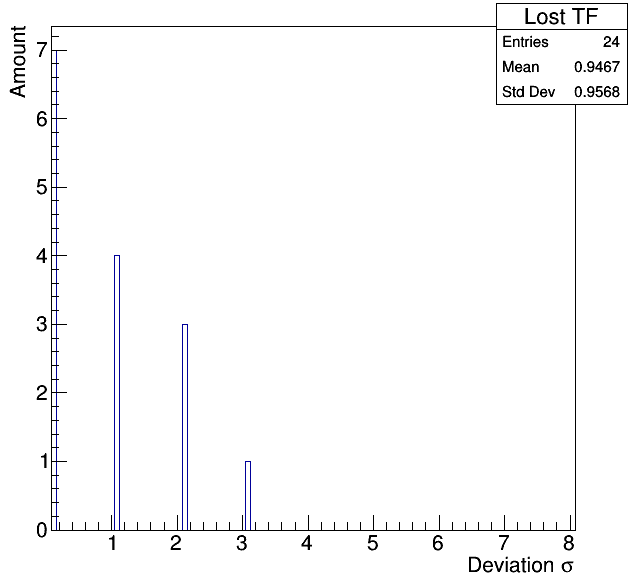
\includegraphics[scale=0.5]{./graphics/ex2_histogram.png}
	\caption{Histogram of the TF lost for ticktime 5}
	\label{Ex2Histogram}
\end{figure}

\newpage

\section{Ex.3 2 FLPs 12 EPNs}
\textbf{Ticktime influence on the Blacklist algorithm with all but one-fail over with random sample size.}
\\~\\
Compliant with the previous results, the TF loss to ticktime ratio rises in a linear line, with no absurdities along the way. The amounts are also negligibly different to the previous results. Results can be seen in table ~\ref{table:Ex3MitchResults} and table ~\ref{table:Ex3HeikoResults}. A histogram for ticktime 5 can be seen at ~\ref{fig:Ex3Histogram}. It shows a standard deviation of 1.569 for all the TFs lost in the entire run. 

\begin{table}[h!]
\caption*{\textbf{Experiment three (2/12) using a cluster of Raspberry Pi's}}
\resizebox{\textwidth}{!}{\begin{tabular}{| p{0.1\linewidth} | >{\centering}m{0.7cm} | >{\centering}m{0.7cm} | >{\centering}m{0.7cm} | >{\centering}m{0.7cm} | >{\centering}m{0.7cm} | >{\centering}m{0.7cm} | >{\centering}m{0.7cm} | >{\centering}m{0.7cm} | >{\centering}m{0.7cm} | >{\centering}m{0.7cm} | >{\centering}m{0.7cm} | >{\centering}m{0.7cm} |}
\hline
Lost EPNs & 1 EPN & 2 EPNs & 3 EPNs & 4 EPNs & 5 EPNs & 6 EPNs & 7 EPNs & 8 EPNs & 9 EPNs & 10 EPNs & 11 EPNs & Total \tabularnewline \hline
Ticktime &&&&&&&&&&&& \tabularnewline \hline
5 & 1.92 & 1.96 & 1.96 & 2.2 & 2.52 & 2.88 & 2.96 & 3.08 & 3.56 & 4.2 & 4.92 & \textbf{23.88}\tabularnewline \hline
10 & 1.96 & 2.3 & 2.52 & 2.74 & 2.81 & 2.93 & 2.85 & 3.48 & 3.85 & 4.74 & 6.33 & \textbf{26.52}\tabularnewline \hline
15 & 3 & 2.92 & 2.96 & 2.96 & 3.21 & 3.38 & 4.04 & 4.42 & 5.25 & 6.29 & 8.67 & \textbf{37.08}\tabularnewline \hline
20 & 3 & 3 & 3.38 & 3.5 & 3.92 & 4.17 & 4.79 & 5.17 & 6.08 & 7.54 & 10.88 & \textbf{45.12}\tabularnewline \hline
25 & 3.71 & 3.54 & 3.92 & 3.83 & 4.13 & 4.79 & 5.33 & 6.13 & 7.21 & 9.17 & 13.38 & \textbf{55.13}\tabularnewline \hline
\end{tabular}}
\caption{Cumulative lost TFs by ticktime/EPN ratio with a random sample size for the Blacklist algorithm}
\label{table:Ex3MitchResults}
\end{table}

\begin{table}[htb]
\caption*{\textbf{Experiment three (2/12) using a cluster on Nikhef}}
\resizebox{\textwidth}{!}{\begin{tabular}{| p{0.1\linewidth} | >{\centering}m{0.7cm} | >{\centering}m{0.7cm} | >{\centering}m{0.7cm} | >{\centering}m{0.7cm} | >{\centering}m{0.7cm} | >{\centering}m{0.7cm} | >{\centering}m{0.7cm} | >{\centering}m{0.7cm} | >{\centering}m{0.7cm} | >{\centering}m{0.7cm} | >{\centering}m{0.7cm} |}
\hline
Lost EPNs & 1 EPN & 2 EPNs & 3 EPNs & 4 EPNs & 5 EPNs & 6 EPNs & 7 EPNs & 8 EPNs & 9 EPNs & 10 EPNs & 11 EPNs \tabularnewline \hline
Ticktime &&&&&&&&&&& \tabularnewline \hline
5 & 1 & 2 & 2 & 2 & 2 & 3 & 3 & 3 & 3 & 4 & 4 \tabularnewline \hline
10 & 1 & 3 & 3 & 3 & 3 & 3 & 3 & 4 & 4 & 5 & 6 \tabularnewline \hline
15 & 11 & 3 & 3 & 3 & 3 & 3 & 4 & 4 & 5 & 6 & 7 \tabularnewline \hline
20 & 10 & 3 & 3 & 3 & 4 & 4 & 4 & 5 & 6 & 7 & 9 \tabularnewline \hline
25 & 13 & 3 & 4 & 4 & 4 & 4 & 5 & 5 & 7 & 8 & 10 \tabularnewline \hline
\end{tabular}}
\caption{Cumulative TF data loss across events with the Blacklist algorithm and a random sample size (van der Heijden, 2018, p. 40)} 
\label{table:Ex3HeikoResults}
\end{table}

\begin{figure}
	\centering
	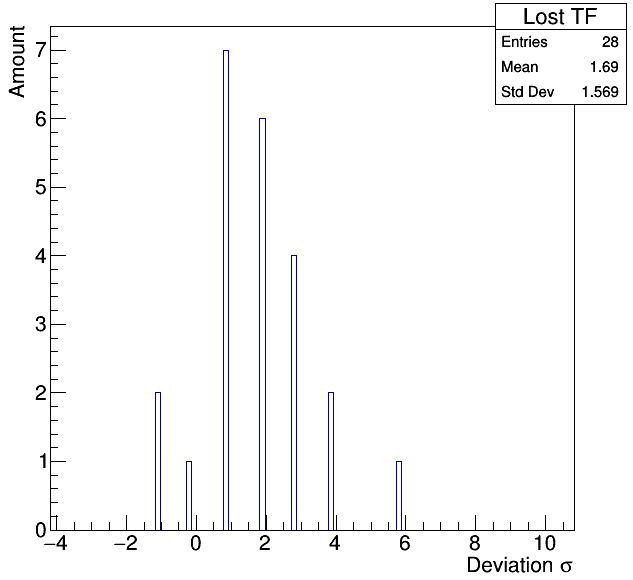
\includegraphics[scale=0.5]{./graphics/ex3_histogram.png}
	\caption{Histogram of the TF loss for ticktime 5}
	\label{fig:Ex3Histogram}
\end{figure}

\newpage

\section{Ex.1 3 FLPs 18 EPNs}
\textbf{Ticktime influence on the Blacklist algorithm with one fail-over.}
\\~\\
The results of the experiment are shown in table ~\ref{table:Ex1318Results}. It shows a linear line going up. At ticktime 10 there is only an average of 1 TF loss. This is the 1 TF that is lost when a shutdown is initialized. These results are lower compared to the results in table ~\ref{table:Ex1MitchResults}.

\begin{table}[h!]
\caption*{\textbf{Experiment one (3/18) using a cluster of Raspberry Pi's}}
\begin{tabular}{| l | l | l |}
\hline
Ticktime & Mean TF loss & Standard Deviation \\ \hline
5 & 1.13 & 0.34 \\ \hline
10 & 1 & 0 \\ \hline
15 & 1.92 & 0.50 \\ \hline
20 & 2.08 & 0.28 \\ \hline
25 & 2.08 & 0.28 \\ \hline
30 & 2.08 & 0.28 \\ \hline
35 & 2.52 & 0.51 \\ \hline
40 & 2.84 & 0.37 \\ \hline
\end{tabular}
\caption{Results of the TFs lost with 1 fail over using a cluster of Raspberry Pi's}
\label{table:Ex1318Results}
\end{table}

\newpage

\section{Ex.2 3 FLPs 18 EPNs}
\textbf{Ticktime influence on the Blacklist algorithm with all but one fail-over.}
\\~\\
The results of the experiment are shown in ~\ref{table:Ex2318Results}. It shows a lower TF loss compared to ~\ref{table:Ex2MitchResults}. It shows that at a ticktime of 5, every fail over will have a TF loss of < 2. This 1 TF comes from the shutdown signal. This means that the time between shutdown, and coming back around again to the EPN, is longer than the time needed to refresh the blacklist. 

\begin{table}[h!]
\caption*{\textbf{Experiment two (3/18) using a cluster of Raspberry Pi's}}
\resizebox{\textwidth}{!}{\begin{tabular}{| p{0.1\linewidth} | >{\centering}m{0.7cm} | >{\centering}m{0.7cm} | >{\centering}m{0.7cm} | >{\centering}m{0.7cm} | >{\centering}m{0.7cm} | >{\centering}m{0.7cm} | >{\centering}m{0.7cm} | >{\centering}m{0.7cm} | >{\centering}m{0.7cm} | >{\centering}m{0.7cm} | >{\centering}m{0.7cm} | >{\centering}m{0.7cm} |}
\hline
Lost EPNs & 1 EPN & 2 EPNs & 3 EPNs & 4 EPNs & 5 EPNs & 6 EPNs & 7 EPNs & 8 EPNs & 9 EPNs & 10 EPNs & 11 EPNs & Total \tabularnewline \hline
Ticktime &&&&&&&&&&&& \tabularnewline \hline
5 & 1.14 & 1.1 & 1.05 & 1.05 & 1.05 & 1.1 & 1.5 & 1 & 1.67 & 1.52 & 1.62 & \textbf{3.33}\tabularnewline \hline
10 & 1.04 & 1.25 & 1.29 & 1.17 & 1.88 & 2.04 & 2 & 2.08 & 1.96 & 2.08 & 2.04 & \textbf{8.83} \tabularnewline \hline
15 & 2 & 2.08 & 2.08 & 2.08 & 2.04 & 2 & 2.08 & 2.08 & 2.33 & 2.71 & 2.79 & \textbf{14.29}\tabularnewline \hline
20 & 2.16 & 2.12 & 2.08 & 2.08 & 2.16 & 2.12 & 2.4 & 2.52 & 2.96 & 3.04 & 3.08 & \textbf{16.72}\tabularnewline \hline
25 & 2.04 & 2.16 & 2.04 & 2.16 & 2.6 & 2.48 & 2.92 & 3.08 & 3.2 & 3.36 & 3.72 & \textbf{19.76}\tabularnewline \hline
\end{tabular}}
\caption{Cumulative lost TFs by ticktime/EPN ratio with a flat sample size for the Blacklist algorithm}
\label{table:Ex2318Results}
\end{table}

\section{Ex.3 3 FLPs 18 EPNs}
\textbf{Ticktime influence on the Blacklist algorithm with all but one-fail over with random sample size.}
\\~\\

The results of the experiment are shown in table ~\ref{table:Ex3318Results}. Oddly enough these results show a more sine wave in the data loss. All these results are again lower compared to ~\ref{table:Ex3MitchResults}.

\begin{table}[h!]
\caption*{\textbf{Experiment three (3/18) using a cluster of Raspberry Pi's}}
\resizebox{\textwidth}{!}{\begin{tabular}{| p{0.1\linewidth} | >{\centering}m{0.7cm} | >{\centering}m{0.7cm} | >{\centering}m{0.7cm} | >{\centering}m{0.7cm} | >{\centering}m{0.7cm} | >{\centering}m{0.7cm} | >{\centering}m{0.7cm} | >{\centering}m{0.7cm} | >{\centering}m{0.7cm} | >{\centering}m{0.7cm} | >{\centering}m{0.7cm} | >{\centering}m{0.7cm} |}
\hline
Lost EPNs & 1 EPN & 2 EPNs & 3 EPNs & 4 EPNs & 5 EPNs & 6 EPNs & 7 EPNs & 8 EPNs & 9 EPNs & 10 EPNs & 11 EPNs & Total \tabularnewline \hline
Ticktime &&&&&&&&&&&& \tabularnewline \hline
5 & 2.56 & 2.39 & 2.22 & 1.17 & 1.22 & 2 & 1.11 & 2.17 & 1.44 & 1.33 & 1.72 & \textbf{9.33}\tabularnewline \hline
10 & 2.88 & 2.88 & 2.38 & 1.08 & 1.71 & 2 & 1.54 & 2.25 & 2.08 & 2 & 2.29 & \textbf{13.08}\tabularnewline \hline
15 & 3.08 & 4 & 3 & 2.04 & 2.04 & 2.58 & 2.08 & 3.04 & 2.33 & 2.25 & 2.54 & \textbf{19}\tabularnewline \hline
20 & 3.28 & 4.04 & 3.24 & 2.08 & 2.12 & 3.12 & 2.16 & 3.16 & 3 & 2.88 & 3.08 & \textbf{22.16}\tabularnewline \hline
25 & 3.7 & 4.09 & 3.87 & 2.52 & 2.78 & 3.13 & 2.83 & 3.65 & 3.39 & 3.3 & 3.96 & \textbf{27.22}\tabularnewline \hline
\end{tabular}}
\caption{Cumulative lost TFs by ticktime/EPN ratio with a random sample size for the Blacklist algorithm}
\label{table:Ex3318Results}
\end{table}

\newpage

\section{Ex.1 4 FLPs 24 EPNs}
\textbf{Ticktime influence on the Blacklist algorithm with one fail-over.}
\\~\\

\begin{table}[h!]
\caption*{\textbf{Experiment one (4/24) using a cluster of Raspberry Pi's}}
\begin{tabular}{| l | l | l |}
\hline
Ticktime & Mean TF loss & Standard Deviation \\ \hline
5 & 1 & 0 \\ \hline
10 & 1.08 & 0.28 \\ \hline
15 & 1.76 & 0.53 \\ \hline
20 & 2.12 & 0.44 \\ \hline
25 & 2 & 0 \\ \hline
30 & 2 & 0 \\ \hline
35 & 2.16 & 0.37 \\ \hline
40 & 2.33 & 0.48 \\ \hline
\end{tabular}
\caption{Results of the TFs lost with 1 fail over using a cluster of Raspberry Pi's}
\label{table:Ex1424Results}
\end{table}

\section{Ex.2 4 FLPs 24 EPNs}
\textbf{Ticktime influence on the Blacklist algorithm with all but one fail-over.}
\\~\\
Table ~\ref{table:Ex1424Results} shows the results of the experiment. It shows a the same linear line going up per EPN as in the previous experiments. These results are yet again smaller than the results from table ~\ref{table:Ex1318Results}.

\begin{table}[h!]
\caption*{\textbf{Experiment two (4/24) using a cluster of Raspberry Pi's}}
\resizebox{\textwidth}{!}{\begin{tabular}{| p{0.1\linewidth} | >{\centering}m{0.7cm} | >{\centering}m{0.7cm} | >{\centering}m{0.7cm} | >{\centering}m{0.7cm} | >{\centering}m{0.7cm} | >{\centering}m{0.7cm} | >{\centering}m{0.7cm} | >{\centering}m{0.7cm} | >{\centering}m{0.7cm} | >{\centering}m{0.7cm} | >{\centering}m{0.7cm} | >{\centering}m{0.7cm} |}
\hline
Lost EPNs & 1 EPN & 2 EPNs & 3 EPNs & 4 EPNs & 5 EPNs & 6 EPNs & 7 EPNs & 8 EPNs & 9 EPNs & 10 EPNs & 11 EPNs & Total \tabularnewline \hline
Ticktime &&&&&&&&&&&& \tabularnewline \hline
5 & 1.15 & 1.15 & 1.25 & 1.15 & 1.05 & 1.15 & 1.15 & 1.15 & 1.1 & 1.1 & 1.25 & \textbf{2.65}\tabularnewline \hline
10 & 1.08 & 1.04 & 1.08 & 1.08 & 1.48 & 1.48 & 1.52 & 1.8 & 2.04 & 1.96 & 2.24 & \textbf{6.8} \tabularnewline \hline
15 & 1.4 & 1.68 & 1.72 & 2 & 2.04 & 2.04 & 2.08 & 2 & 2.08 & 2 & 2.08 & \textbf{11.12}\tabularnewline \hline
20 & 2.12 & 2.04 & 2.08 & 2 & 2.16 & 2.12 & 2.08 & 2.08 & 2.12 & 2.08 & 2.24 & \textbf{13.12}\tabularnewline \hline
25 & 2.12 & 2.12 & 2.16 & 2.12 & 2.12 & 2.04 & 2.2 & 2.08 & 2.6 & 2.68 & 2.64 & \textbf{14.88}\tabularnewline \hline
\end{tabular}}
\caption{Cumulative lost TFs by ticktime/EPN ratio with a flat sample size for the Blacklist algorithm}
\label{table:Ex2424Results}
\end{table}

\section{Ex.3 4 FLPs 24 EPNs}
\textbf{Ticktime influence on the Blacklist algorithm with all but one fail-over with random sample size.}
\\~\\

\begin{table}[h!]
\caption*{\textbf{Experiment three (4/24) using a cluster of Raspberry Pi's}}
\resizebox{\textwidth}{!}{\begin{tabular}{| p{0.1\linewidth} | >{\centering}m{0.7cm} | >{\centering}m{0.7cm} | >{\centering}m{0.7cm} | >{\centering}m{0.7cm} | >{\centering}m{0.7cm} | >{\centering}m{0.7cm} | >{\centering}m{0.7cm} | >{\centering}m{0.7cm} | >{\centering}m{0.7cm} | >{\centering}m{0.7cm} | >{\centering}m{0.7cm} | >{\centering}m{0.7cm} |}
\hline
Lost EPNs & 1 EPN & 2 EPNs & 3 EPNs & 4 EPNs & 5 EPNs & 6 EPNs & 7 EPNs & 8 EPNs & 9 EPNs & 10 EPNs & 11 EPNs & Total \tabularnewline \hline
Ticktime &&&&&&&&&&&& \tabularnewline \hline
5 & 1.1 & 2.14 & 1.14 & 1.57 & 1.24 & 2.14 & 1.14 & 2 & 2.1 & 1.48 & 2.05 & \textbf{8.1}\tabularnewline \hline
10 & 1.52 & 1.96 & 1.04 & 1.68 & 1.4 & 2.04 & 1.36 & 1.88 & 2.04 & 2.04 & 2.16 & \textbf{9.12}\tabularnewline \hline
15 & 2.08 & 2.04 & 1.04 & 2.16 & 2.16 & 2.4 & 2.12 & 1.92 & 2.12 & 2.08 & 2.28 & \textbf{12.4}\tabularnewline \hline
20 & 2.04 & 2.2 & 1.48 & 2.32 & 2.16 & 2.88 & 2.04 & 2.8 & 2.96 & 2.2 & 2.96 & \textbf{16.04}\tabularnewline \hline
25 & 2.13 & 2.54 & 2.08 & 2.33 & 2.33 & 3.13 & 2.13 & 2.96 & 3 & 2.92 & 3.04 & \textbf{18.58}\tabularnewline \hline
\end{tabular}}
\caption{Cumulative lost TFs by ticktime/EPN ratio with a random sample size for the Blacklist algorithm}
\label{table:Ex3424Results}
\end{table}

\section{Ex.4 4 FLPs 24 EPNs}
\textbf{Ticktime influence on the Blacklist algorithm with a fixed cluster fail-over pattern using a random sample size.}
\\~\\
Table ~\ref{table:Ex4424Results} shows the results of the experiment. It shows that for the first 4 clusters the TF loss is low, but for the last cluster it's substantially higher. Because of this, the total average is also a lot higher.

\begin{table}[h!]
\caption*{\textbf{Experiment four (4/24) using a cluster of Raspberry Pi's}}
\resizebox{\textwidth}{!}{\begin{tabular}{| >{\centering}m{2cm} | >{\centering}m{2cm} | >{\centering}m{2cm} | >{\centering}m{2cm} | >{\centering}m{2cm} | >{\centering}m{2cm} | >{\centering}m{2cm} |}
\hline
Lost Clusters & 1 Cluster & 2 Clusters & 3 Clusters & 4 Clusters & 5 Clusters & Total \tabularnewline \hline
Ticktime &&&&&& \tabularnewline \hline
5 & 2.83 & 5.25 & 1.88 & 4.67 & 250.67 & \textbf{261.29}\tabularnewline \hline
10 & 3.64 & 3.76 & 6.04 & 4.52 & 285.92 & \textbf{299.88}\tabularnewline \hline
15 & 5.6 & 2.04 & 6.28 & 7.76 & 277.68 & \textbf{295.36}\tabularnewline \hline
20 & 7.26 & 4.74 & 6.26 & 13.3 & 296.09 & \textbf{323.65}\tabularnewline \hline
25 & 7.44 & 8.4 & 8.12 & 9.44 & 254.72 & \textbf{284.12}\tabularnewline \hline
\end{tabular}}
\caption{Cumulative lost TFs by ticktime/EPN ratio with a random sample size for the Blacklist algorithm and a fixed cluster 	fail-over pattern}
\label{table:Ex4424Results}
\end{table}

\section{Ex.5 4 FLPs 24EPNs}
\textbf{Ticktime influence on the Blacklist algorithm with a random cluster fail-over pattern using a random sample size}
\\~\\
Table ~\ref{table:Ex5424Results} shows the result of the experiment. It shows that with a random cluster fail-over pattern, the total average TF loss is close to the results in table ~\ref{table:Ex4424Results}, but for each seperate cluster they are higher. Unlike the previous experiment where it's all lower numbers first and then finally a very large one.

\begin{table}[h!]
\caption*{\textbf{Experiment five (4/24) using a cluster of Raspberry Pi's}}
\resizebox{\textwidth}{!}{\begin{tabular}{| >{\centering}m{2cm} | >{\centering}m{2cm} | >{\centering}m{2cm} | >{\centering}m{2cm} | >{\centering}m{2cm} | >{\centering}m{2cm} | >{\centering}m{2cm} |}
\hline
Lost Clusters & 1 Cluster & 2 Clusters & 3 Clusters & 4 Clusters & 5 Clusters & Total \tabularnewline \hline
Ticktime &&&&&& \tabularnewline \hline
5 & 3.21 & 23.53 & 38.32 & 79.53 & 174.89 & \textbf{315.47}\tabularnewline \hline
10 & 4.48 & 21.92 & 35.36 & 40.44 & 185.04 & \textbf{283.24}\tabularnewline \hline
15 & 5.52 & 23 & 36.84 & 28.16 & 188.4 & \textbf{277.92}\tabularnewline \hline
20 & 5.68 & 24.8 & 39.6 & 42.52 & 190.64 & \textbf{299.24}\tabularnewline \hline
25 & 6.26 & 26.74 & 42.83 & 84.61 & 194.39 & \textbf{350.83}\tabularnewline \hline
\end{tabular}}
\caption{Cumulative lost TFs by ticktime/EPN ratio with a random sample size for the Blacklist algorithm and a fixed cluster 	fail-over pattern}
\label{table:Ex5424Results}
\end{table}

\section{Analysis}
\subsection{Comparison to the previous experiment}
To calculate the validity of the results, the Pearson correlation will be used. This is calculated using:\\
\begin{flalign*}
\hspace*{-5cm} \rho x,y = \frac{\sum (x-m_{x})(y-m_{y})}{\sqrt{\sum(x-m_{x})^2(y-m_{y})^2}}
\end{flalign*}

~\\ Where $m_{x}$ is the mean of vector $x$, and $m_{y}$ is the mean of vector $y$.
~\\ A way to calculate this in python is shown in listing ~\ref{lst:PearsonInPython} The results of this can be found in table ~\ref{table:PearsonCor}. The totals of all separate tests are combined to calculate this correlation.

\begin{lstlisting}[frame=single,language=Python,caption={Pearson correlation calculation in Python},label={lst:PearsonInPython}]
from scipy.stats.stats import pearsonr
def list of values X
def list of values Y
pearsonr(X,Y)
\end{lstlisting}

\begin{table}[h!]
\begin{tabular}{| l | l | l |}
\hline
Experiment & Pearson Correlation \\ \hline
1 & 0.95 \\ \hline
2 & 0.99 \\ \hline
3 & 0.99 \\ \hline
\end{tabular}
\caption{Pearson correlation between the raspberry pi cluster and the cluster on Nikhef}
\label{table:PearsonCor}
\end{table}

~\\ These correlations all strongly deny the null hypothesis, and thus there is some sort of statistical relationship. They also are close to 1, which means they are close to having a total positive linear correlation. Thus concluded that there is indeed a correlation between the setup on Nikhef, and the setup using Raspberry Pi's.

\subsection{Increasing the numbers of FLPs and EPNs}

When comparing the data between the experiments, the t-test method is used. A way to implement a t-test analysis in Python is shown in listing ~\ref{lst:t-testinInPython}. For every increase in units the t-test will be performed.

\begin{lstlisting}[frame=single,language=Python,caption={t-test analysis in Python},label={lst:t-testinInPython}]
from scipy.stats import ttest_ind
def list of values X
def list of values Y
print ttest_ind(X, Y, equal_var=False)
\end{lstlisting}

\subsubsection*{Correlation between 2/12 and 3/18}
Table ~\ref{table:Ttest23} shows that 

\begin{table}[h!]
\begin{tabular}{| l | l | l |}
\hline
Experiment & t-statistic & p-value \\ \hline
1 & 3.53 & 0.004 \\ \hline
2 & 3.53 & 0.014 \\ \hline
3 & 2.93 & 0.025 \\ \hline
\end{tabular}
\caption{t-test results of the experiments 2/12 and 3/18}
\label{table:Ttest23}
\end{table}

\subsubsection*{Correlation between 3/18 and 4/24}
Table ~\ref{table:Ttest34} shows that 

\begin{table}[h!]
\begin{tabular}{| l | l | l |}
\hline
Experiment & t-statistic & p-value \\ \hline
1 & 0.53 & 0.605 \\ \hline
2 & 0.78 & 0.458 \\ \hline
3 & 1.41 & 0.202 \\ \hline
\end{tabular}
\caption{t-test results of the experiments 3/18 and 4/24}
\label{table:Ttest34}
\end{table}

\subsubsection*{Correlation between 2/12 and 4/24}
Table ~\ref{table:Ttest24} shows that 

\begin{table}[h!]
\begin{tabular}{| l | l | l |}
\hline
Experiment & t-statistic & p-value \\ \hline
1 & 4.15 & 0.002 \\ \hline
2 & 4.09 & 0.010 \\ \hline
3 & 4.02 & 0.010 \\ \hline
\end{tabular}
\caption{t-test results of the experiments 2/12 and 4/24}
\label{table:Ttest24}
\end{table}


\subsection{Comparing cluster fail-over patterns}
For comparing the two experiments the same t-test will be used. The results are shown in ~\ref{table:Ttest45}. It shows that the t-statistic is -0.75 and the p-value is 0.474. This means that there is no significant statistical difference. Looking at the results it shows that that experiment four has lower values for the first four cluster fail-overs, but then has a higher value for the last cluster fail-over, whereas experiment five has higher values overall for each cluster fail-over. This shows that there is a difference in the lost TFs per individual cluster that has a fail-over depending on the layout, but that in the end the total amount is still similar.

\begin{table}[h!]
\begin{tabular}{| l | l | l | l | l |}
\hline
Ticktime & Experiment 4 & Experiment 5 & t-statistic & p-value \\ \hline
5 & 261.29 & 315.47 &  &  \\ \hline
10 & 299.88 & 283.24 &  &  \\ \hline
15 & 295.36 & 277.92 &  &  \\ \hline
20 & 323.65 & 299.24 &  &  \\ \hline
25 & 284.23 & 350.83 &  &  \\ \hline \hline
Total &  &  & \textbf{-0.75} & \textbf{0.474}\\ \hline
\end{tabular}
\caption{t-test results of experiment four and five}
\label{table:Ttest45}
\end{table}

\chapter{Conclusion}

%\section{Conclusion}
The new setup is a viable way of conducting experiments for testing load balancing algorithms. With a Pearson correlation value of 0.95 and higher for the three experiments, we can conclude that there is a very strong positive linear correlation. Further more looking at the data for the expansion of the experiment, we can see that the Information Node does not have a negative effect with handling the extra units. In fact, because it has more time to handle the units in between round robins, less TFs are lost in the process. \\
Lastly, there is a difference in the amount of TFs lost depending on the layout of the system. With each cluster fail-over With the Blacklist algorithm there will be a higher TF loss if the IPs of the machines that have a fail-over are more spread out, as compared to the IPs being one after another. 

\section{Recommendations}
\subsection{Do the experiment with Ansible induced fail-overs}
Both these experiments are done with fail-overs that were induced using the TF that was send at that point. This means that the fail-overs are in a sense predictable, and means that there will always be atleast one TF lost. It is recommended to create scripts that induce a fail-over using Ansible at random time intervals. This to prevent having the one certain TF loss, and to randomize the moment when an EPN will have a fail-over.
\subsection{Use a lowest latency approach, as opposed to a round robin for the distribution}
Currently the distribution is done using a Round Robin approach. This means that the distribution will go from the top of the list, to the bottom each time. This means that if there is a fail-over induced by a TF, it will have the entire list still as a buffer to be targeted again. If there is a lowest latency approach used, then the Information Node will target the EPN that is best suited at the time to receive the TF. If there is a fail-over happening at some point, then this EPN won't be targeted anymore by default.

\chapter{Bibliography}


~~ CERN, 2012, ALICE, online accessed at April 25, retrieved from \\https://home.cern/about/experiments/alice\\

CERN, 2012, About CERN, online accessed at April 25, retrieved from \\https://home.cern/about\\

FairRoot, n.d., About FairRoot, online accessed at April 24, retrieved from \\https://fairroot.gsi.de/?q=about\\

FairRootGroup, 2018, FairRootGroup/FairRoot, online accessed at April 24, retrieved from \\https://github.com/FairRootGroup/FairRoot\\

Raspberry, 2018, Raspberry Pi 3 Model B+, online accessed at April 26, retrieved from \\https://www.raspberrypi.org/products/raspberry-pi-3-model-b-plus/\\

Ansible, Red Hat Ansible, n.d., IT Automation with Ansible, online accessed at April 25, retrieved from \\https://www.ansible.com/overview/it-automation\\

Juniper, 2017, EX3400 Ethernet Switch, online accesed at May 9, retrieved from \\https://www.juniper.net/assets/us/en/local/pdf/datasheets/1000581-en.pdf\\

Tp-Link, 2017, 5-Port 10/100Mbps Desktop Switch TL-SF1005D, online accesed at May 9, retrieved from \\https://www.tp-link.com/us/products/details/cat-5581 TL-SF1005D.html\\

SoftwareForScience, 2018, SoftwareForScience/O2-Balancer, online accessed at April 23, retrieved from \\https://github.com/SoftwareForScience/O2-Balancer\\

Technical design report for the upgrade of the online offline computing system, 2015, The ALICE Collaboration\\

StatSoft Inc, 2013, Electronic Statistics Textbook. online accessed at May 23, retrieved from  \\http://www.statsoft.com/textbook/statistics-glossary/p\# Pearson\%20Correlation

\appendix
\addcontentsline{toc}{chapter}{Appendices}
\chapter*{Appendices}
\renewcommand{\thesection}{\Alph{section}}
\section{Glossary}
%\section{Glossary}
\begin{table}[htb]
\resizebox{\textwidth}{!}{\begin{tabular}{l|c|r}
Term & Abbreviation & Meaning \\ \hline
CERN & & European association for nuclear research \\
LHC & Large Hardon Collider & Largest particle collider  at CERN used for researching matter \\
ALICE & A Large Ion Collider Experiment & Detector on the LHC for detecting quark-gluon plasma \\
IN & Information Node & Computer that runs manages all the underlying computers \\
FLP & First Level Processor & The first computer in line for receiving data \\
EPN & Event Processing Node & Last computer in line that stores all the data received \\
STF & Sub Time Frame & Data from the detector \\ 
TF & Time Frame & Compressed data from 2 STFs \\
Fail-Over & & An event where an EPN is disabled \\
FairRoot & & A simulation framework based on ROOT \\
FairMQ & & The data transport layer of FairRoot \\
Zookeeper & & A service for maintaining information and configurations of units \\
Ticktime & & The time in ms that Zookeeper uses to update \\
Ansible & &  Deployment software for IT infrastructures \\
Blacklist & & An algorithm that maintains a list of targets to work with
\end{tabular}}
\end{table}
\section{Planning}
%\documentclass{report}
%\usepackage[utf8]{inputenc}
%\usepackage{longtable}

%\begin{document}

%\section{Planning as of 25/04/2018}
\begin{longtable}{| p{0.22\linewidth} | p{0.3\linewidth}| p{0.2\linewidth} | l | l |}
\hline
\textbf{Name} & \textbf{Description} & \textbf{Deliverable} & \textbf{Est.} & \textbf{Complete} \\ \hline

Create scripts for all experiments & Create all the scripts for the deployment of experiments & Experiment scripts & 6 hours & 19/04/2018 \\
\hline

Experiment 1 (2/12) & Ticktime influence on the blacklist algorithm with one fail-over & Compressed Ex.1 2/12 results & 105 hours & 30/04/2018 \\ 
\hline

Experiment 2 (2/12) & Ticktime influence on the blacklist algorithm with all but one fail-over & Compressed Ex.2 2/12 results & 19 hours & 01/05/2018 \\
\hline

Work out Ex.1 (2/12) & Compile results of Ex.1 (2/12) & Compiled results of Ex.1 (2/12) & 2 hours & 30/04/2018 \\
\hline  

Write chapter 6.1 & Write down the results for chapter 6.1 about the results of Ex.1 (2/12) & Chapter 6.1 & 3 hours & 30/04/2018 \\
\hline

Experiment 3 (2/12) & Ticktime influence on the blacklist algorithm with all but one-fail over with random sample size & Compressed Ex.3 2/12 results & 19 hours & 02/05/2018 \\
\hline

Work out Ex.2 (2/12) & Compile results of Ex.2 (2/12) & Compiled results of Ex.2 (2/12) & 2 hours & 01/05/2018 \\
\hline 

Write chapter 6.2 & Write down the results for chapter 6.2 about the results of Ex.2 (2/12) & Chapter 6.2 & 3 hours & 01/05/2018 \\
\hline

Experiment 2 (3/18) & Ticktime influence on the blacklist algorithm with all but one fail-over & Compressed Ex.2 3/18 results & 19 hours & 03/05/2018 \\
\hline

Work out Ex.3 (2/12) & Compile results of Ex.3 (2/12) & Compiled results of Ex.3 (2/12) & 2 hours & 02/05/2018 \\
\hline

Write chapter 6.3 & Write down the results for chapter 6.3 about the results of Ex.3 (2/12) & Chapter 6.3 & 3 hours & 02/05/2018 \\
\hline

Experiment 2 (4/24) & Ticktime influence on the blacklist algorithm with all but one fail-over & Compressed Ex.2 4/24 results & 19 hours & 04/05/2018 \\
\hline

Work out Ex.2 (3/18) & Compile results of Ex.2 (3/18) & Compiled results of Ex.2 (3/18) & 2 hours & 03/05/2018 \\
\hline
 
Write chapter 6.5 & Write down the results for chapter 6.5 about the results of Ex.2 (3/18) & Chapter 6.5 & 3 hours & 03/05/2018 \\
\hline

Experiment 3 (3/18) & Ticktime influence on the blacklist algorithm with all but one-fail over with random sample size & Compressed Ex.3 3/18 results & 19 hours & 09/05/2018 \\
\hline

Work out Ex.2 (4/24) & Compile results of Ex.2 (4/24) & Compiled results of Ex.2 (4/24) & 2 hours & 04/05/2018 \\
\hline 

Write chapter 6.8 & Write down the results for chapter 6.8 about the results of Ex.2 (4/24) & Chapter 6.8 & 3 hours & 04/05/2018 \\
\hline

Experiment 3 (4/24) & Ticktime influence on the blacklist algorithm with all but one-fail over with random sample size & Compressed Ex.3 4/24 results & 19 hours & 10/05/2018 \\
\hline

Work out Ex.3 (3/18) & Compile results of Ex.3 (3/18) & Compiled results of Ex.3 (3/18) & 2 hours & 09/05/2018 \\
\hline 

Write chapter 6.6 & Write down the results for chapter 6.6 about the results of Ex.3 (3/18) & Chapter 6.6 & 3 hours & 09/05/2018 \\
\hline

Experiment 1 (3/18) & Ticktime influence on the blacklist algorithm with one fail-over & Compressed Ex.1 3/18 results & 105 hours & 14/05/2018 \\ 
\hline

Work out Ex.3 (4/24) & Compile results of Ex.3 (4/24) & Compiled results of Ex.3 (4/24) & 2 hours & 11/05/2018 \\
\hline 

Write chapter 6.9 & Write down the results for chapter 6.9 about the results of Ex.3 (4/24) & Chapter 6.9 & 3 hours &  11/05/2018 \\
\hline

Experiment 1 (4/24) & Ticktime influence on the blacklist algorithm with one fail-over & Compressed Ex.1 4/24 results & 105 hours & 19/05/2018 \\ 
\hline

Work out Ex.1 (3/18) & Compile results of Ex.1 (3/18) & Compiled results of Ex.1 (3/18) & 2 hours & 15/05/2018 \\
\hline 

Write chapter 6.4 & Write down the results for chapter 6.4 about the results of Ex.1 (3/18) & Chapter 6.4 & 3 hours & 15/05/2018 \\
\hline

Compile + write appendixes & Compile and write down everything that needs to go in the appendix, which include the bibliography, email documentation, and glossary & Appendixes & 4 hours & 16/05/2018 \\
\hline

Work out Ex.1 (4/24) & Compile results of Ex.1 (4/24) & Compiled results of Ex.1 (4/24) & 2 hours & 21/05/2018 \\
\hline 

Write chapter 6.7 & Write down the results for chapter 6.7 about the results of Ex.1 (4/24) & Chapter 6.7 & 3 hours & 21/05/2018 \\
\hline

Write a summary in 2/3 languages & Write a summary of the thesis in English, Dutch and German & Summaries & 16 hours & 18/05/2018 \\
\hline

Experiment 4 (4/24) & Ticktime influence on the blacklist algorithm with all but one fail-over at once & Compressed Ex.4 4/24 results & 19 hours & 22/05/2018 \\
\hline

Work out Ex.4 (4/24) & Compile results of Ex.4 (4/24) & Compiled results of Ex.4 (4/24) & 2 hours & 23/05/2018 \\
\hline

Write chapter 6.10 & Write down the results for chapter 6.10 about the results of Ex.4 (4/24) & Chapter 6.10 & 3 hours & 23/05/2018 \\
\hline

Write a preface & Write a small preface & Preface & 1 hours & 24/05/2018 \\
\hline

Write an introduction & Write an introduction for the thesis & Introduction & 2 hours & 24/05/2018 \\
\hline

Write chapter 7.1 & Write down the conclusions based on the results of the previous experiments & Chapter 7.1 & 3 hours & 25/05/2018 \\
\hline

Write chapter 7.2 & Write down the recommendations based on the results of the previous experiments & Chapter 7.2 & 3 hours & 25/05/2018 \\
\hline

\end{longtable}
%\end{document}

\end{document}